\chapter{Appendix II}
\label{app2}
\section{The coding of the proposed approach}
\large
This Appendix includes the Python codes for running the pipeline. From the codes can be seen the used packages and the code itself is also enriched with inline comments. The actual \textbf{.py} files can be read and/or downloaded from the GitHub repository:

\large
\begin{enumerate}
\item \href{https://github.com/AntigoniKourou/Thesis/blob/master/reviews_sentiment.py}{Reading the reviews and getting their sentiment}
\item \href{https://github.com/AntigoniKourou/Thesis/blob/master/feature_identification.py}{Feature extraction}
\item \href{https://github.com/AntigoniKourou/Thesis/blob/639bc78aa558220cfd515ed9777b4f44aa8c0d7b/language_check.py}{Language check}
\item \href{https://github.com/AntigoniKourou/Thesis/blob/6a938f108fab5dbc39af224a643f57e682777064/lemmatization.py}{Lemmatization}
\item \href{https://github.com/AntigoniKourou/Thesis/blob/5ab99a3da8522858b091ebd8f0c289c4460fc3ee/lemmas.py}{Getting the lemmas of SYNSETs from the ontology}
\end{enumerate}

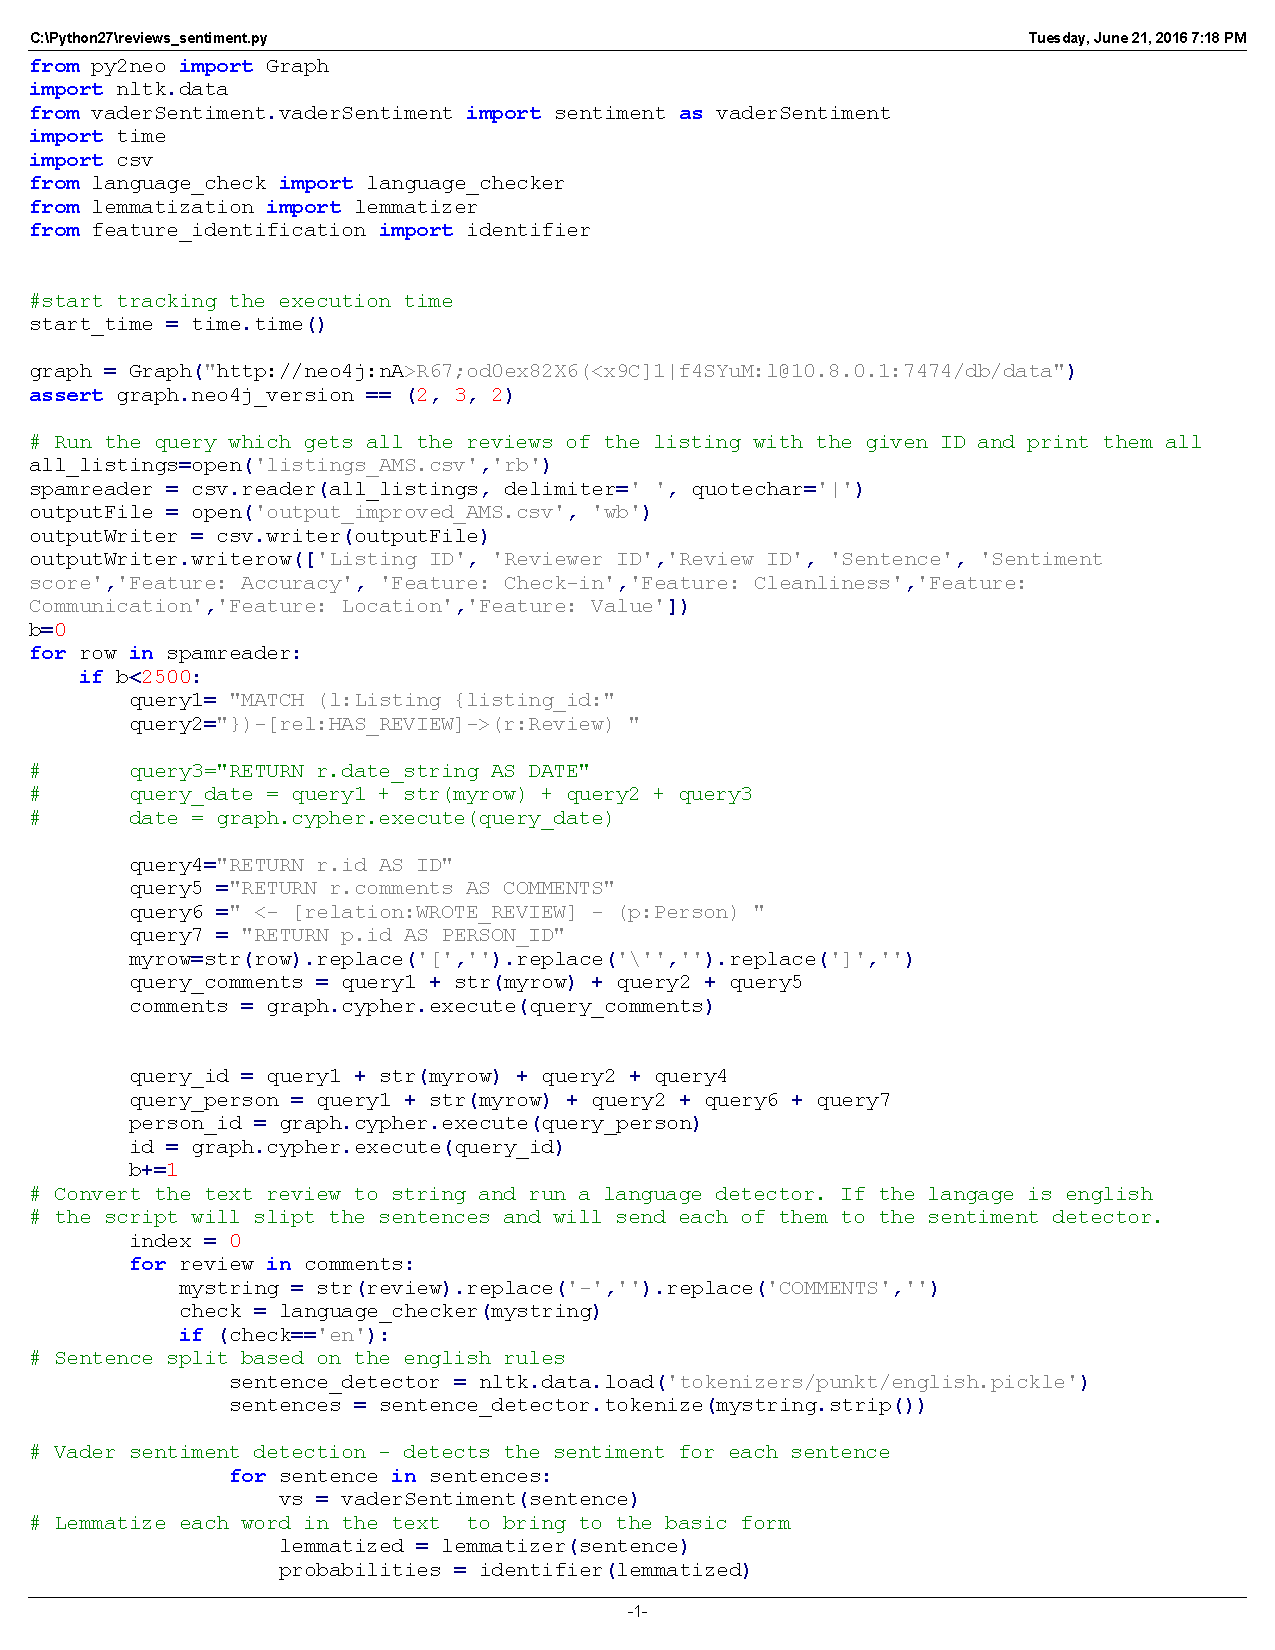
\includepdf[pages={-}]{reviews_sentiment.pdf}
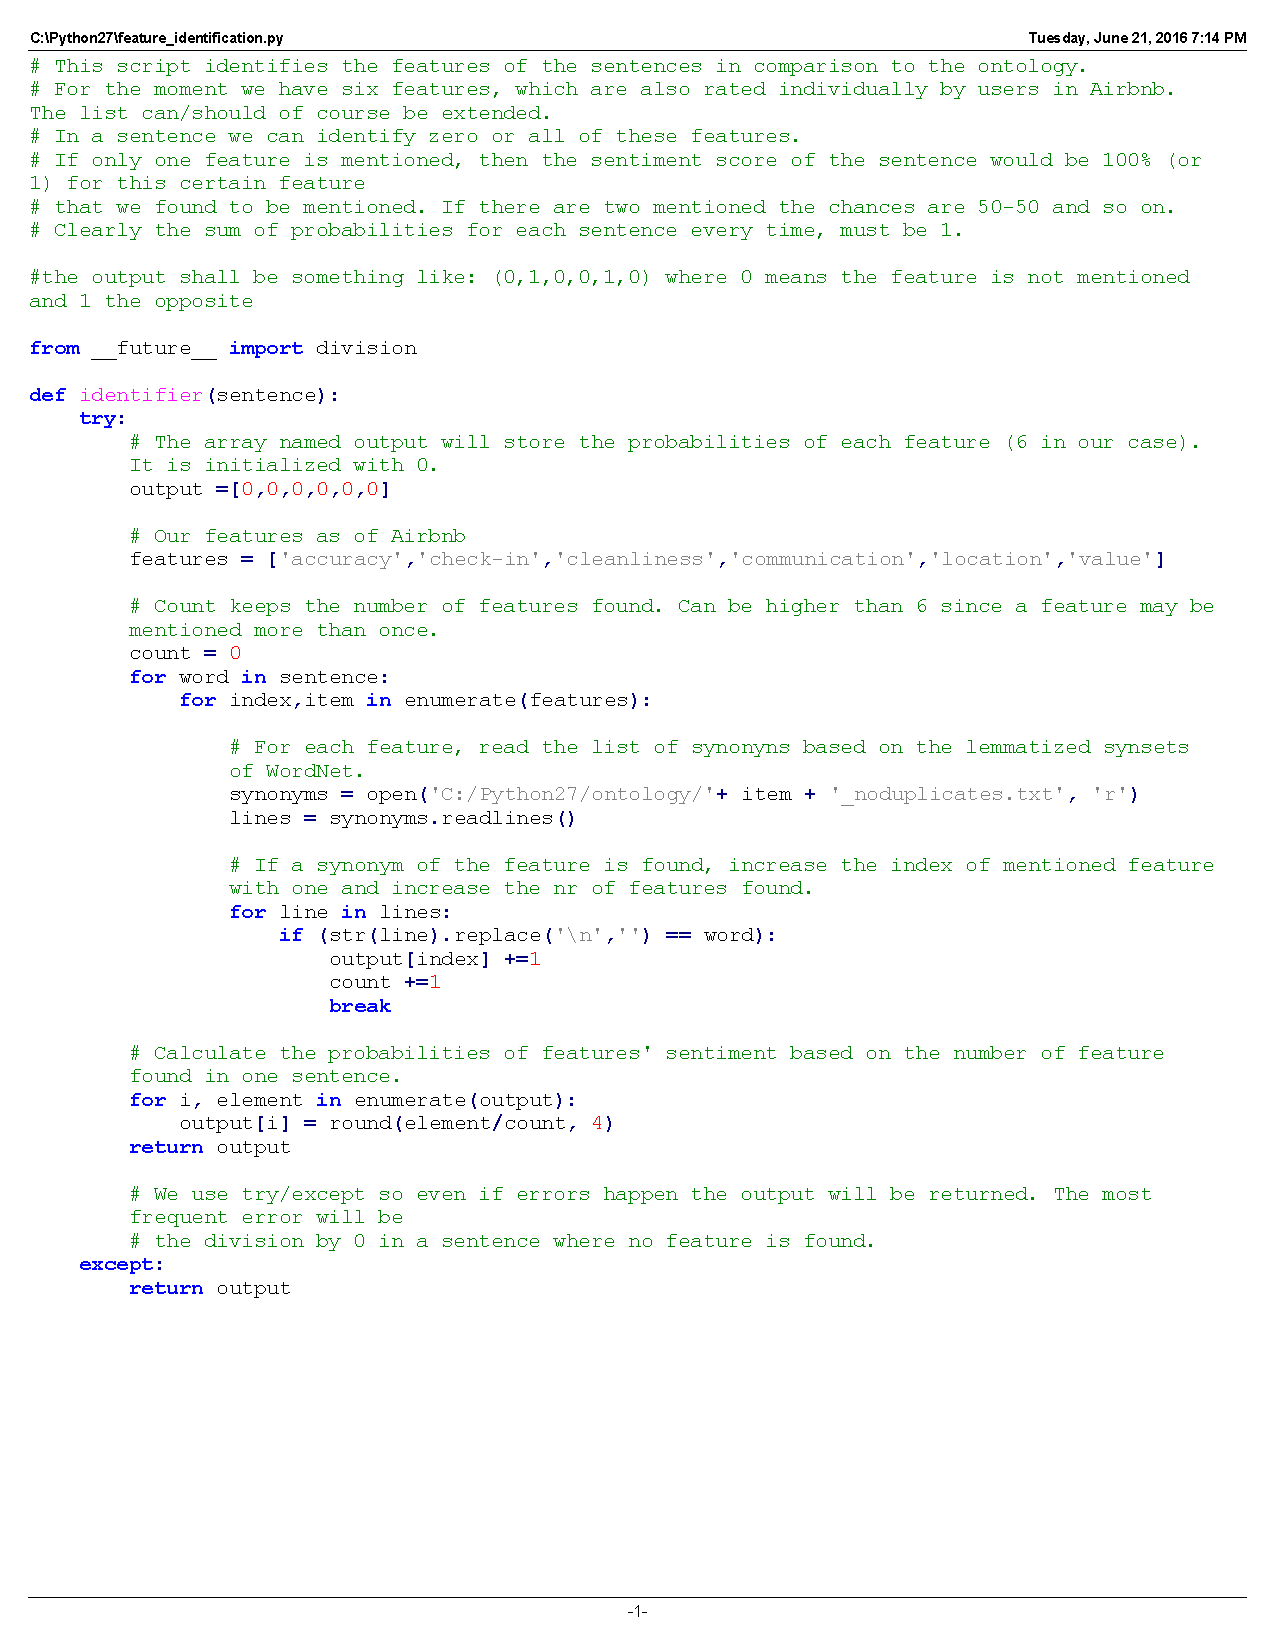
\includepdf[pages={-}]{feature_identification.pdf}
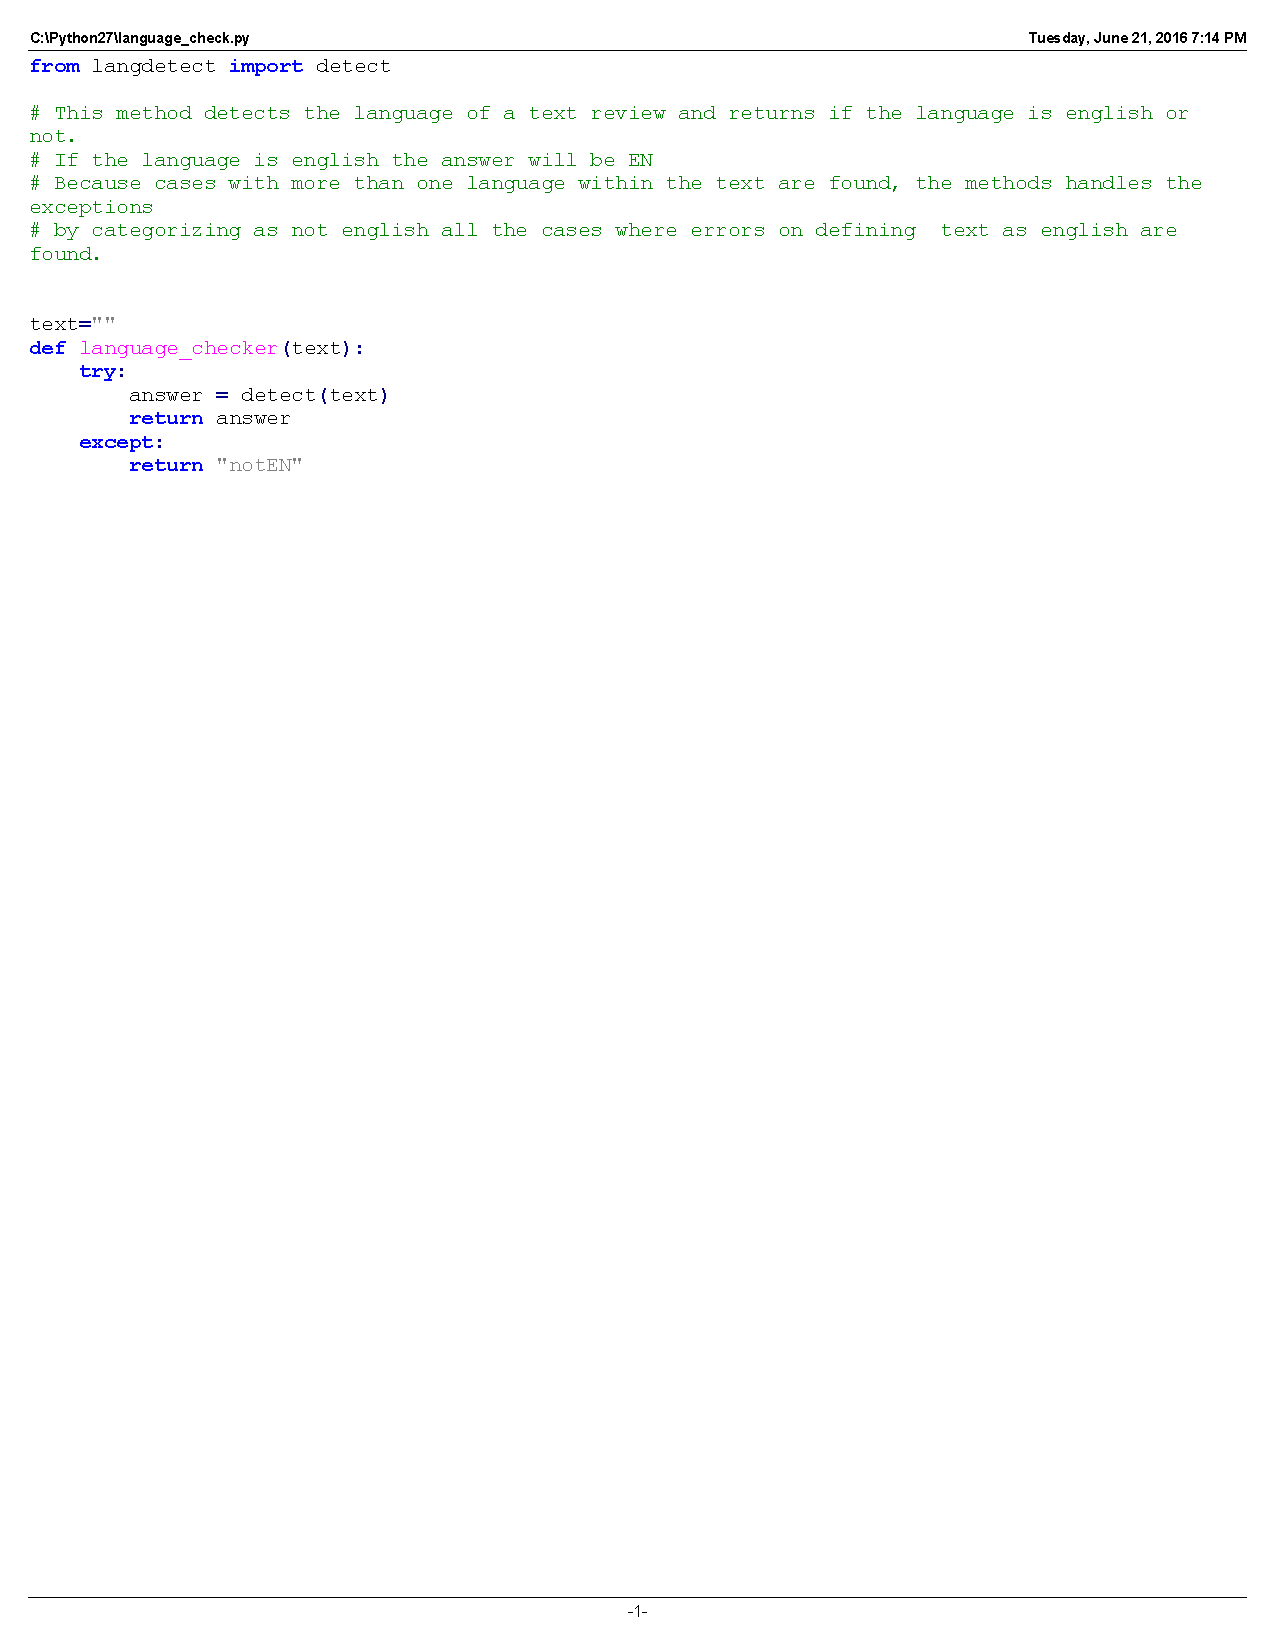
\includepdf[pages={-}]{language_check.pdf}
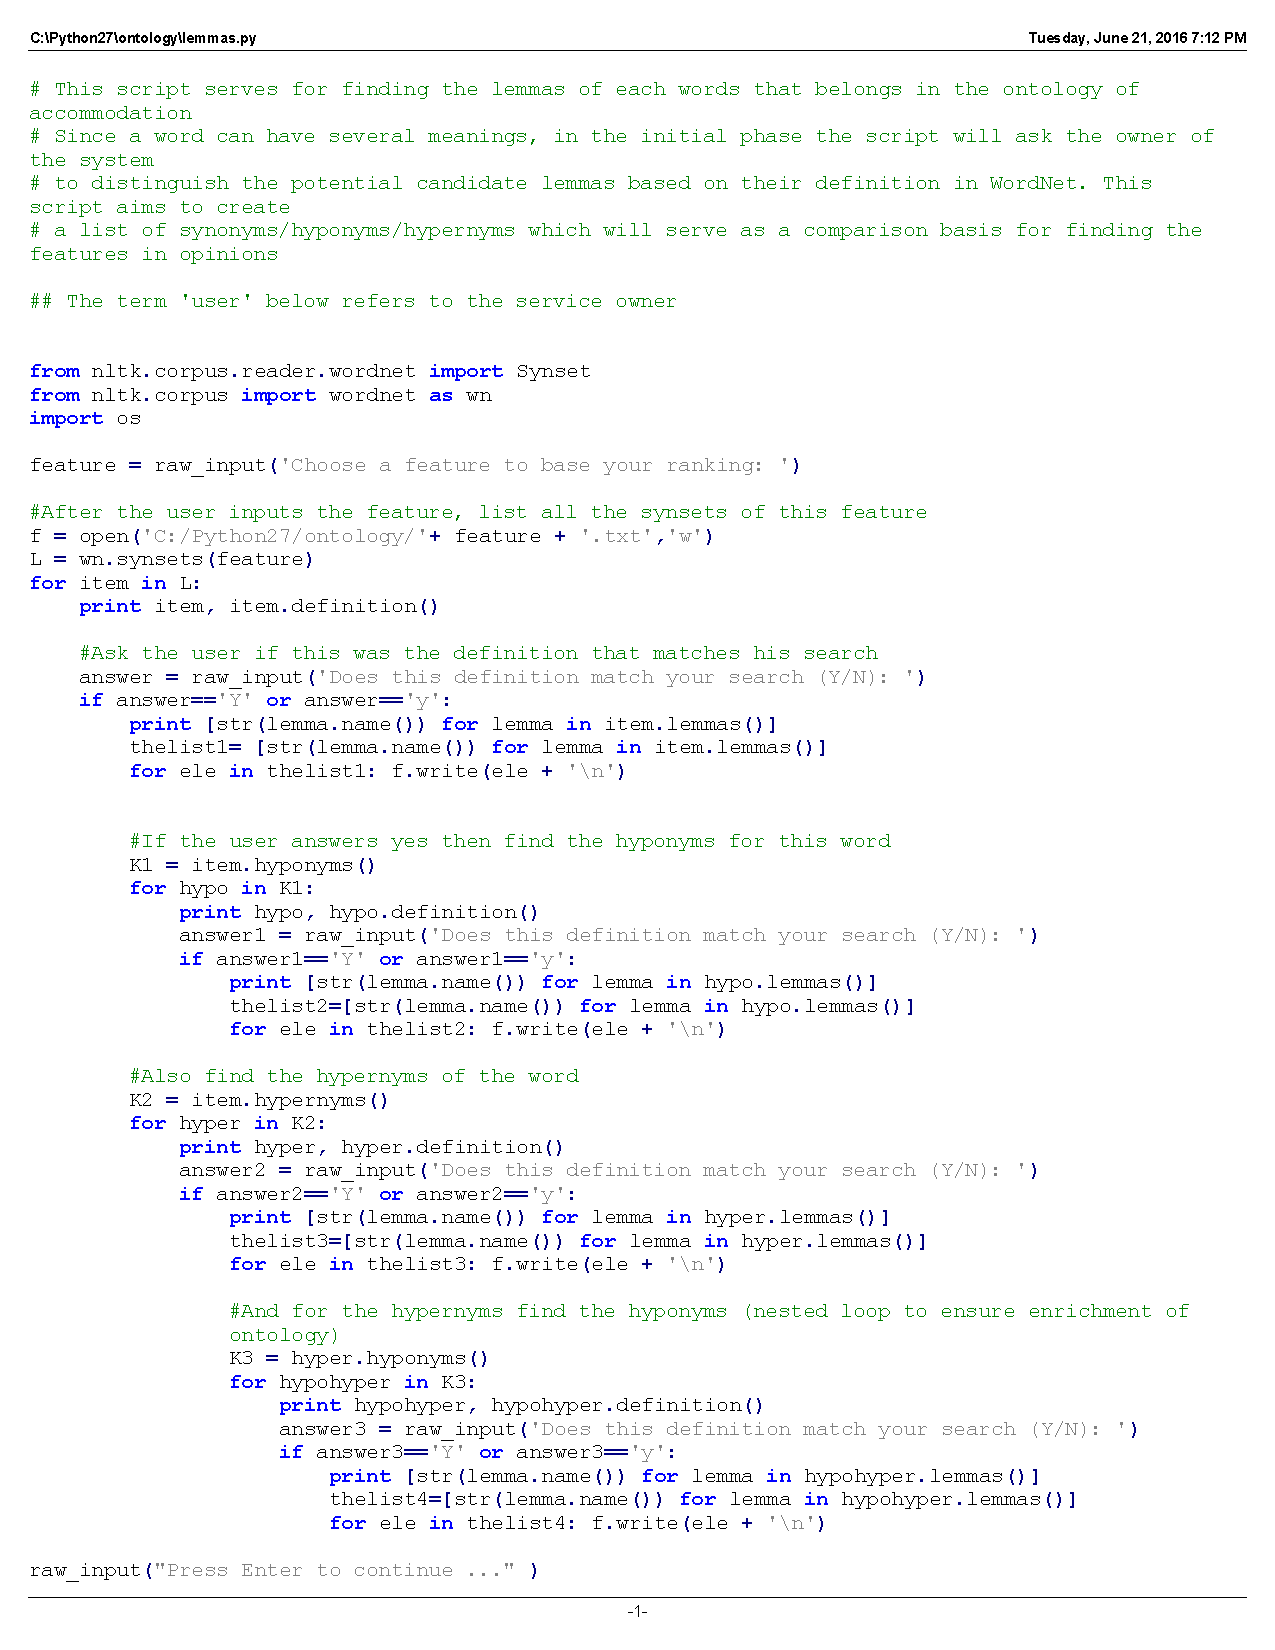
\includepdf[pages={-}]{lemmas.pdf}
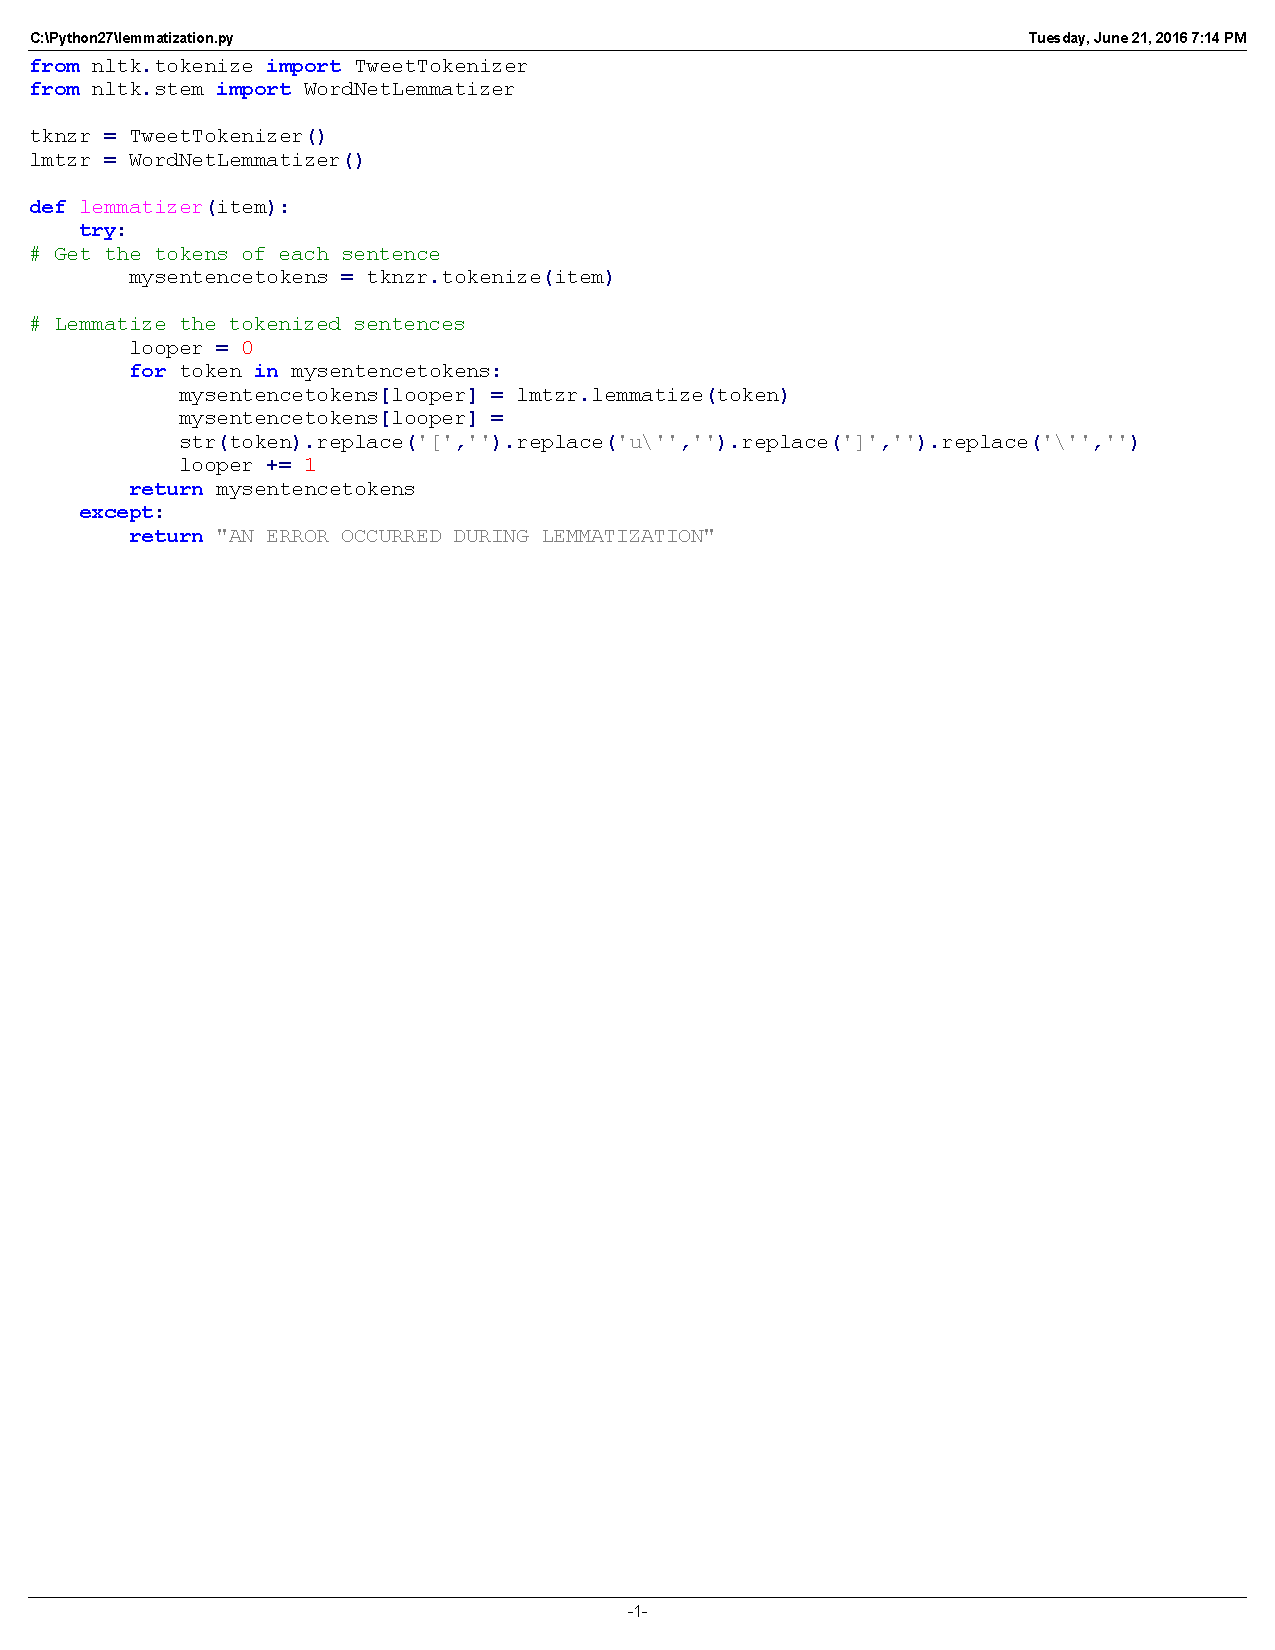
\includepdf[pages={-}]{lemmatization.pdf}